\documentclass[10pt]{article}

\usepackage[margin=0.72in]{geometry}
\usepackage{graphicx}
\usepackage{amsmath}
\usepackage{booktabs}
\usepackage{longtable}
\usepackage{array}
\usepackage{xcolor}
\usepackage{hyperref}
\usepackage{seqsplit}
\usepackage{caption}
\usepackage{float}
\usepackage{microtype}

\hypersetup{
  colorlinks=true,
  linkcolor=blue!60!black,
  urlcolor=blue!60!black,
  citecolor=blue!60!black
}

\newcommand{\bitstr}[1]{\begingroup\ttfamily\footnotesize\seqsplit{#1}\endgroup}
\newcommand{\code}[1]{\texttt{#1}}
\newcommand{\good}{\textcolor{green!45!black}{validated}}
\newcommand{\warn}{\textcolor{orange!70!black}{candidate}}
\newcommand{\bad}{\textcolor{red!65!black}{unreliable}}
\setlength{\tabcolsep}{3pt}
\renewcommand{\arraystretch}{1.08}

\title{\vspace{-1.2em}Quantum Peak Challenge: Session Report}
\author{Local Codex run on \code{quantum-junction}}
\date{6 June 2026}

\begin{document}
\maketitle
\vspace{-1.2em}

\begin{abstract}
This report consolidates the fragmented analysis performed in this session: static QASM forensics, exact statevector baselines, Aer MPS sampling, MPS distillation across seeds and bond dimensions, and the \code{peaked-circuit-simulation} MPO/unswapping attempt.  The central result is that exact simulation validated ten small circuits; approximate methods agreed on most exact-checkable cases but \code{24\_13} exposed a real failure mode of single-qubit marginal thresholding.  For larger circuits, the safest outputs so far are repeated-sample candidates from MPS sampling/distillation, not single marginal-threshold strings.
\end{abstract}

\section{Challenge and Bit Order}
The challenge circuits are peaked: for each QASM circuit, the task is to recover the output bitstring with the largest measurement probability from input state $\lvert 0\cdots 0\rangle$.  The instructions state that Qiskit-style count strings are ordered with the right-most bit corresponding to qubit $q_0$.  All bitstrings in this report use that convention.

The challenge construction described in \code{INSTRUCTIONS.md} hides an RX-encoded target pattern inside identity-like blocks $U_iU_i^\dagger$ and then applies an obfuscation pass.  The most relevant downloaded references were the peaked-circuit construction paper, the Kremer--Dupuis classical MPO/unswapping attack, and a 2D tensor-network sampling paper.  The practical implication for this repo was: exact statevector is reliable only for small $n$, MPS sampling can work when the peak remains strong, and the local \code{peaked-circuit-simulation} implementation is a plausible structural attack but needs careful validation.

\section{Artifacts Produced}
The project environment was installed in the repo and all heavy runs were submitted to Slurm rather than run directly on the login node.  The main output locations are:

\begin{itemize}
  \item \code{agent\_work/exact\_baseline/}: exact Aer statevector results for circuits up to 28 qubits.
  \item \code{agent\_work/static\_forensics/}: QASM metrics, pair repetitions, angle summaries, operation-sequence similarity.
  \item \code{agent\_work/algebraic\_simplify/}: local simplification and Qiskit transpiler probes.
  \item \code{agent\_work/mps\_distill/}: Aer MPS sampling pilot over several seeds, shot counts, and bond dimensions.
  \item \code{outputs/sim\_11\_26\_34\_41\_49/}: requested statevector/MPS runs for challenge IDs 11, 26, 34, 41, and 49, with distribution plots.
  \item \code{outputs/peaked\_circuit\_sim\_pilot/} and \code{outputs/peaked\_circuit\_sim\_all/}: \code{peaked-circuit-simulation} pilot and partial full sweep.
\end{itemize}

\section{Static and Algebraic Analysis}
Static parsing covered all 49 challenge QASM files.  The gate set was only \code{rx}, \code{rz}, \code{cx}, and sparse \code{swap}; no measurements were present in the original challenge files.  Repeated undirected CNOT pairs were common, supporting the inverse-composition hypothesis.  However, local algebraic attacks did not recover the hidden RX pattern.

\begin{figure}[H]
  \centering
  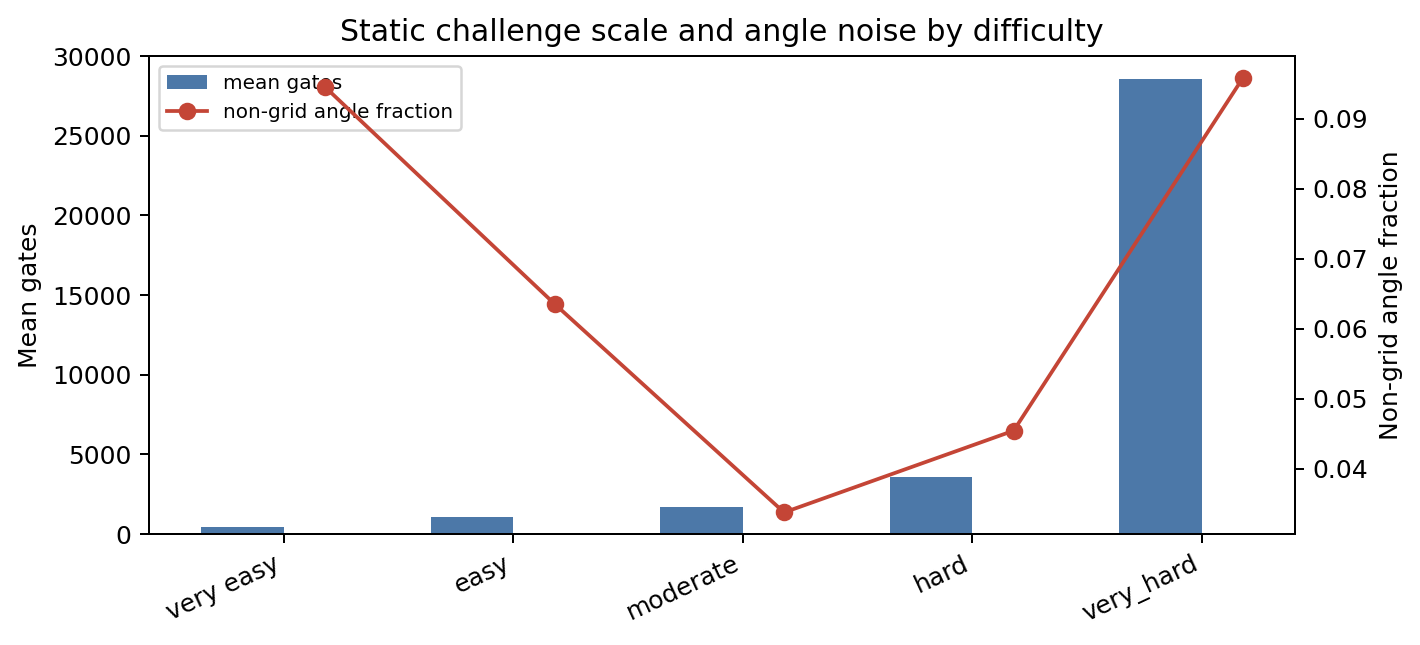
\includegraphics[width=0.78\linewidth]{figures/static_difficulty.png}
  \caption{Static scale by difficulty.  Very-hard circuits are much larger and use a distinct angle-noise profile, consistent with a stronger obfuscation pass.}
\end{figure}

Important negative findings:
\begin{itemize}
  \item Native-basis Qiskit transpilation and adjacent cancellation barely reduced the circuits.
  \item Snapping angles to nearby $\pi$ fractions helped syntax reduction slightly but did not reveal peak bits.
  \item RX($\pi$) remnants, SWAP tracking, and first/trailing RX-layer heuristics failed on small circuits where exact answers were known.
  \item The analysis supports nonlocal or globally dispersed pairings: the cancellations are not adjacent local patterns after obfuscation.
\end{itemize}

\section{Exact Statevector Baseline}
Exact Aer statevector simulation was run for circuits up to 28 qubits.  This produced ten exact peaks and gave a ground truth for validating approximate methods.  Statevector beyond this range was skipped because memory scales as $16\cdot 2^n$ bytes before overhead.

\begin{figure}[H]
  \centering
  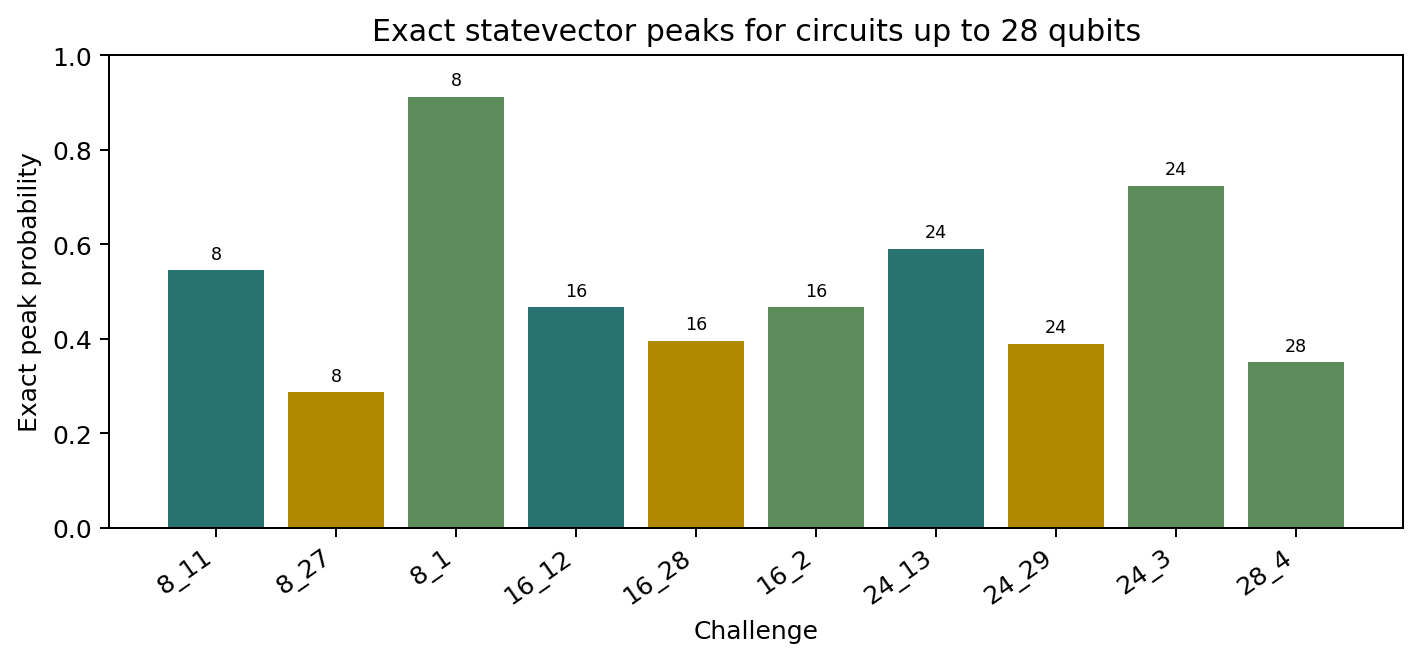
\includegraphics[width=0.82\linewidth]{figures/exact_peak_probabilities.png}
  \caption{Exact peak probabilities for solved small circuits.  The number above each bar is the qubit count.}
\end{figure}

\begin{tabular}{llrp{0.36\linewidth}rr}
\toprule
Challenge & Difficulty & Qubits & Peak bitstring & Peak prob. & Gap \\
\midrule
8\_11 & easy & 8 & \bitstr{01001110} & 0.545448 & 0.476764 \\
8\_27 & moderate & 8 & \bitstr{11001001} & 0.287907 & 0.225213 \\
8\_1 & very easy & 8 & \bitstr{10101101} & 0.912638 & 0.874726 \\
16\_12 & easy & 16 & \bitstr{1111000101101011} & 0.466537 & 0.393572 \\
16\_28 & moderate & 16 & \bitstr{1101001111011100} & 0.396206 & 0.373075 \\
16\_2 & very easy & 16 & \bitstr{1010101011001000} & 0.466970 & 0.369383 \\
24\_13 & easy & 24 & \bitstr{111110011111001011010001} & 0.591248 & 0.544080 \\
24\_29 & moderate & 24 & \bitstr{110100010111100001001001} & 0.390097 & 0.376660 \\
24\_3 & very easy & 24 & \bitstr{011110010000101010001000} & 0.723984 & 0.676891 \\
28\_4 & very easy & 28 & \bitstr{1111111000101010110110011111} & 0.351112 & 0.277609 \\
\bottomrule
\end{tabular}


\section{Aer MPS Sampling and Distillation}
Aer MPS sampling was used in two ways.  First, the requested IDs 11, 26, 34, 41, and 49 were run with statevector where feasible and MPS otherwise.  Second, a pilot distillation grid ran six trials per selected circuit using combinations of \code{shots=512,2048,4096}, \code{bond\_dim=16,32,64}, and two seeds.

\begin{figure}[H]
  \centering
  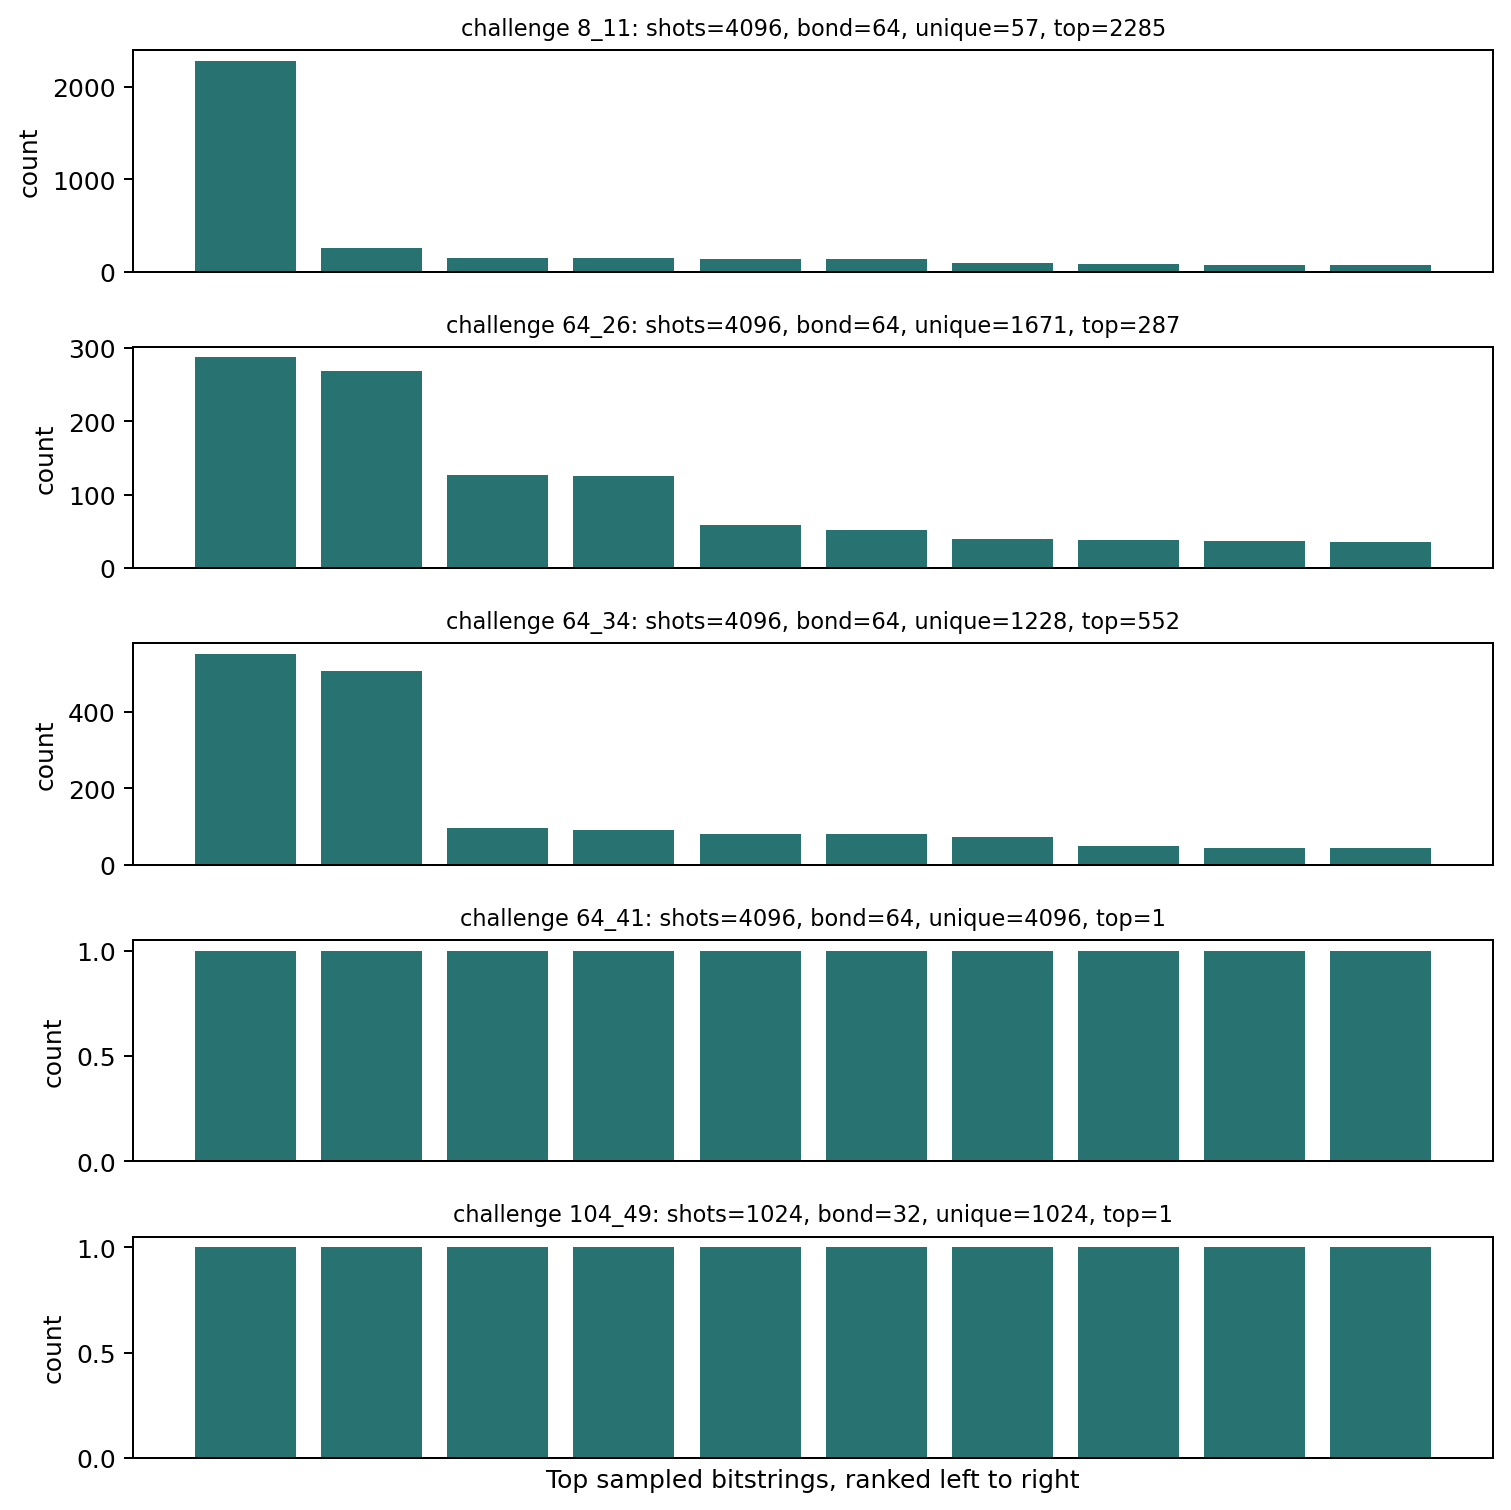
\includegraphics[width=0.86\linewidth]{figures/selected_mps_top_counts.png}
  \caption{Top sampled counts for the requested MPS runs.  IDs 26 and 34 have repeated top samples; IDs 41 and 49 are essentially all-unique samples and therefore low confidence.}
\end{figure}

\begin{figure}[H]
  \centering
  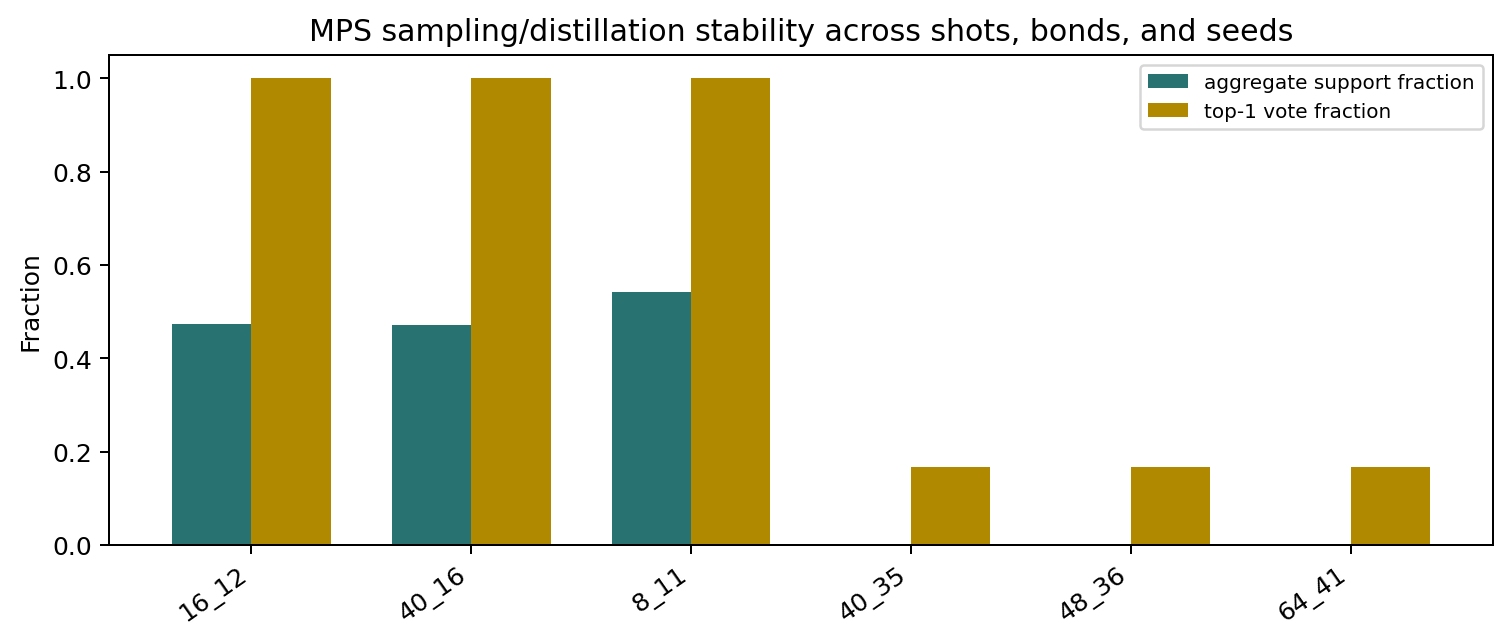
\includegraphics[width=0.78\linewidth]{figures/mps_stability.png}
  \caption{MPS distillation stability.  Easy circuits and \code{40\_16} were stable across seeds/settings; hard pilot circuits were unstable with flat aggregate support.}
\end{figure}

\begin{tabular}{rrrrp{0.43\linewidth}rr}
\toprule
ID & Qubits & Shots & Bond & Top sampled bitstring & Count & Unique \\
\midrule
8\_11 & 8 & 4096 & 64 & \bitstr{01001110} & 2285 & 57 \\
64\_26 & 64 & 4096 & 64 & \bitstr{0110101010100011010111011000011100010110110110011100011001100110} & 287 & 1671 \\
64\_34 & 64 & 4096 & 64 & \bitstr{0011010100010011001110101110100101001011001011011001111011100110} & 552 & 1228 \\
64\_41 & 64 & 4096 & 64 & \bitstr{0011001100010001000101010001110111001000000001011100011011110010} & 1 & 4096 \\
104\_49 & 104 & 1024 & 32 & \bitstr{11100011111110111011110101100011001001100100110010100000001110100001010111101110100010000011010100110101} & 1 & 1024 \\
\bottomrule
\end{tabular}


The MPS distillation summary was the most useful selection rule for non-exact circuits.  For \code{40\_16}, all six trials selected the same candidate and the aggregate support fraction was about 0.471.  For \code{40\_35}, \code{48\_36}, and \code{64\_41}, each top-1 candidate changed across runs and the aggregate winner had support of only two samples; those are not credible answers.

\section{\code{peaked-circuit-simulation} Runs}
The bundled \code{peaked-circuit-simulation} method was adapted through runtime compatibility shims for the installed Qiskit version.  The runner used MPO compression plus unswapping, converted the compressed MPO to an MPS, and extracted a candidate by thresholding one-qubit marginals.

The main parameters used for the full sweep were:
\begin{center}
\code{max\_bond=512}, \code{cutoff=0.002}, \code{unswap\_threshold=1e6}, \code{max\_its=10}, \code{rewire\_trials=64}, \code{seed=123}.
\end{center}
The full sweep was submitted as Slurm job \code{34607501} on \code{interruptible\_gpu}; it produced 21 JSON files before cancellation: 12 completed \code{ok}, 9 remained \code{started}, and 28 challenge outputs were missing.  A retry array \code{34611837} was also cancelled after about three minutes, so no additional retry outputs landed.

\begin{figure}[H]
  \centering
  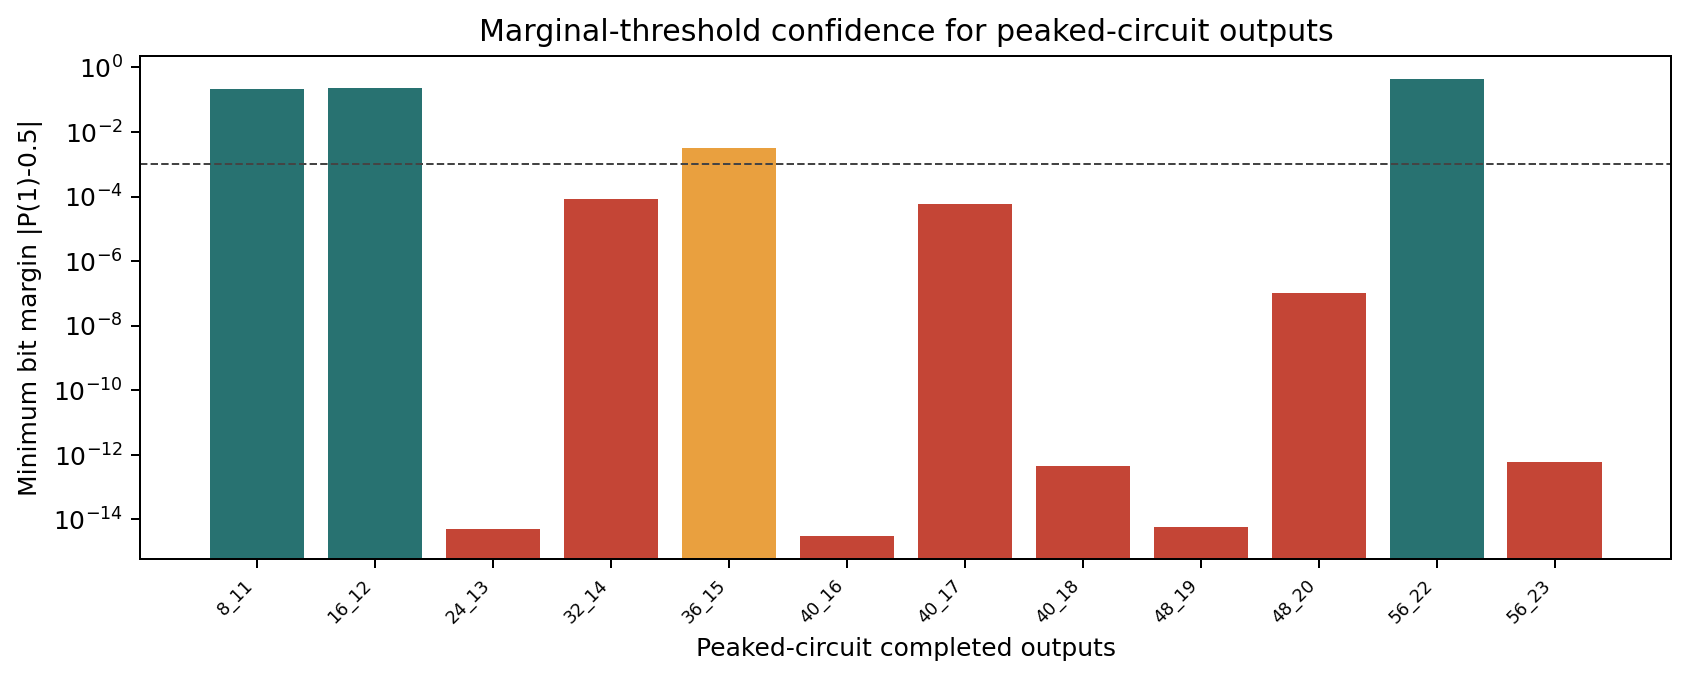
\includegraphics[width=0.86\linewidth]{figures/peaked_margins.png}
  \caption{Confidence of completed \code{peaked-circuit-simulation} outputs.  A small minimum margin means at least one inferred bit was near the $P(1)=0.5$ decision boundary.}
\end{figure}

\begin{figure}[H]
  \centering
  \begin{minipage}{0.32\linewidth}
    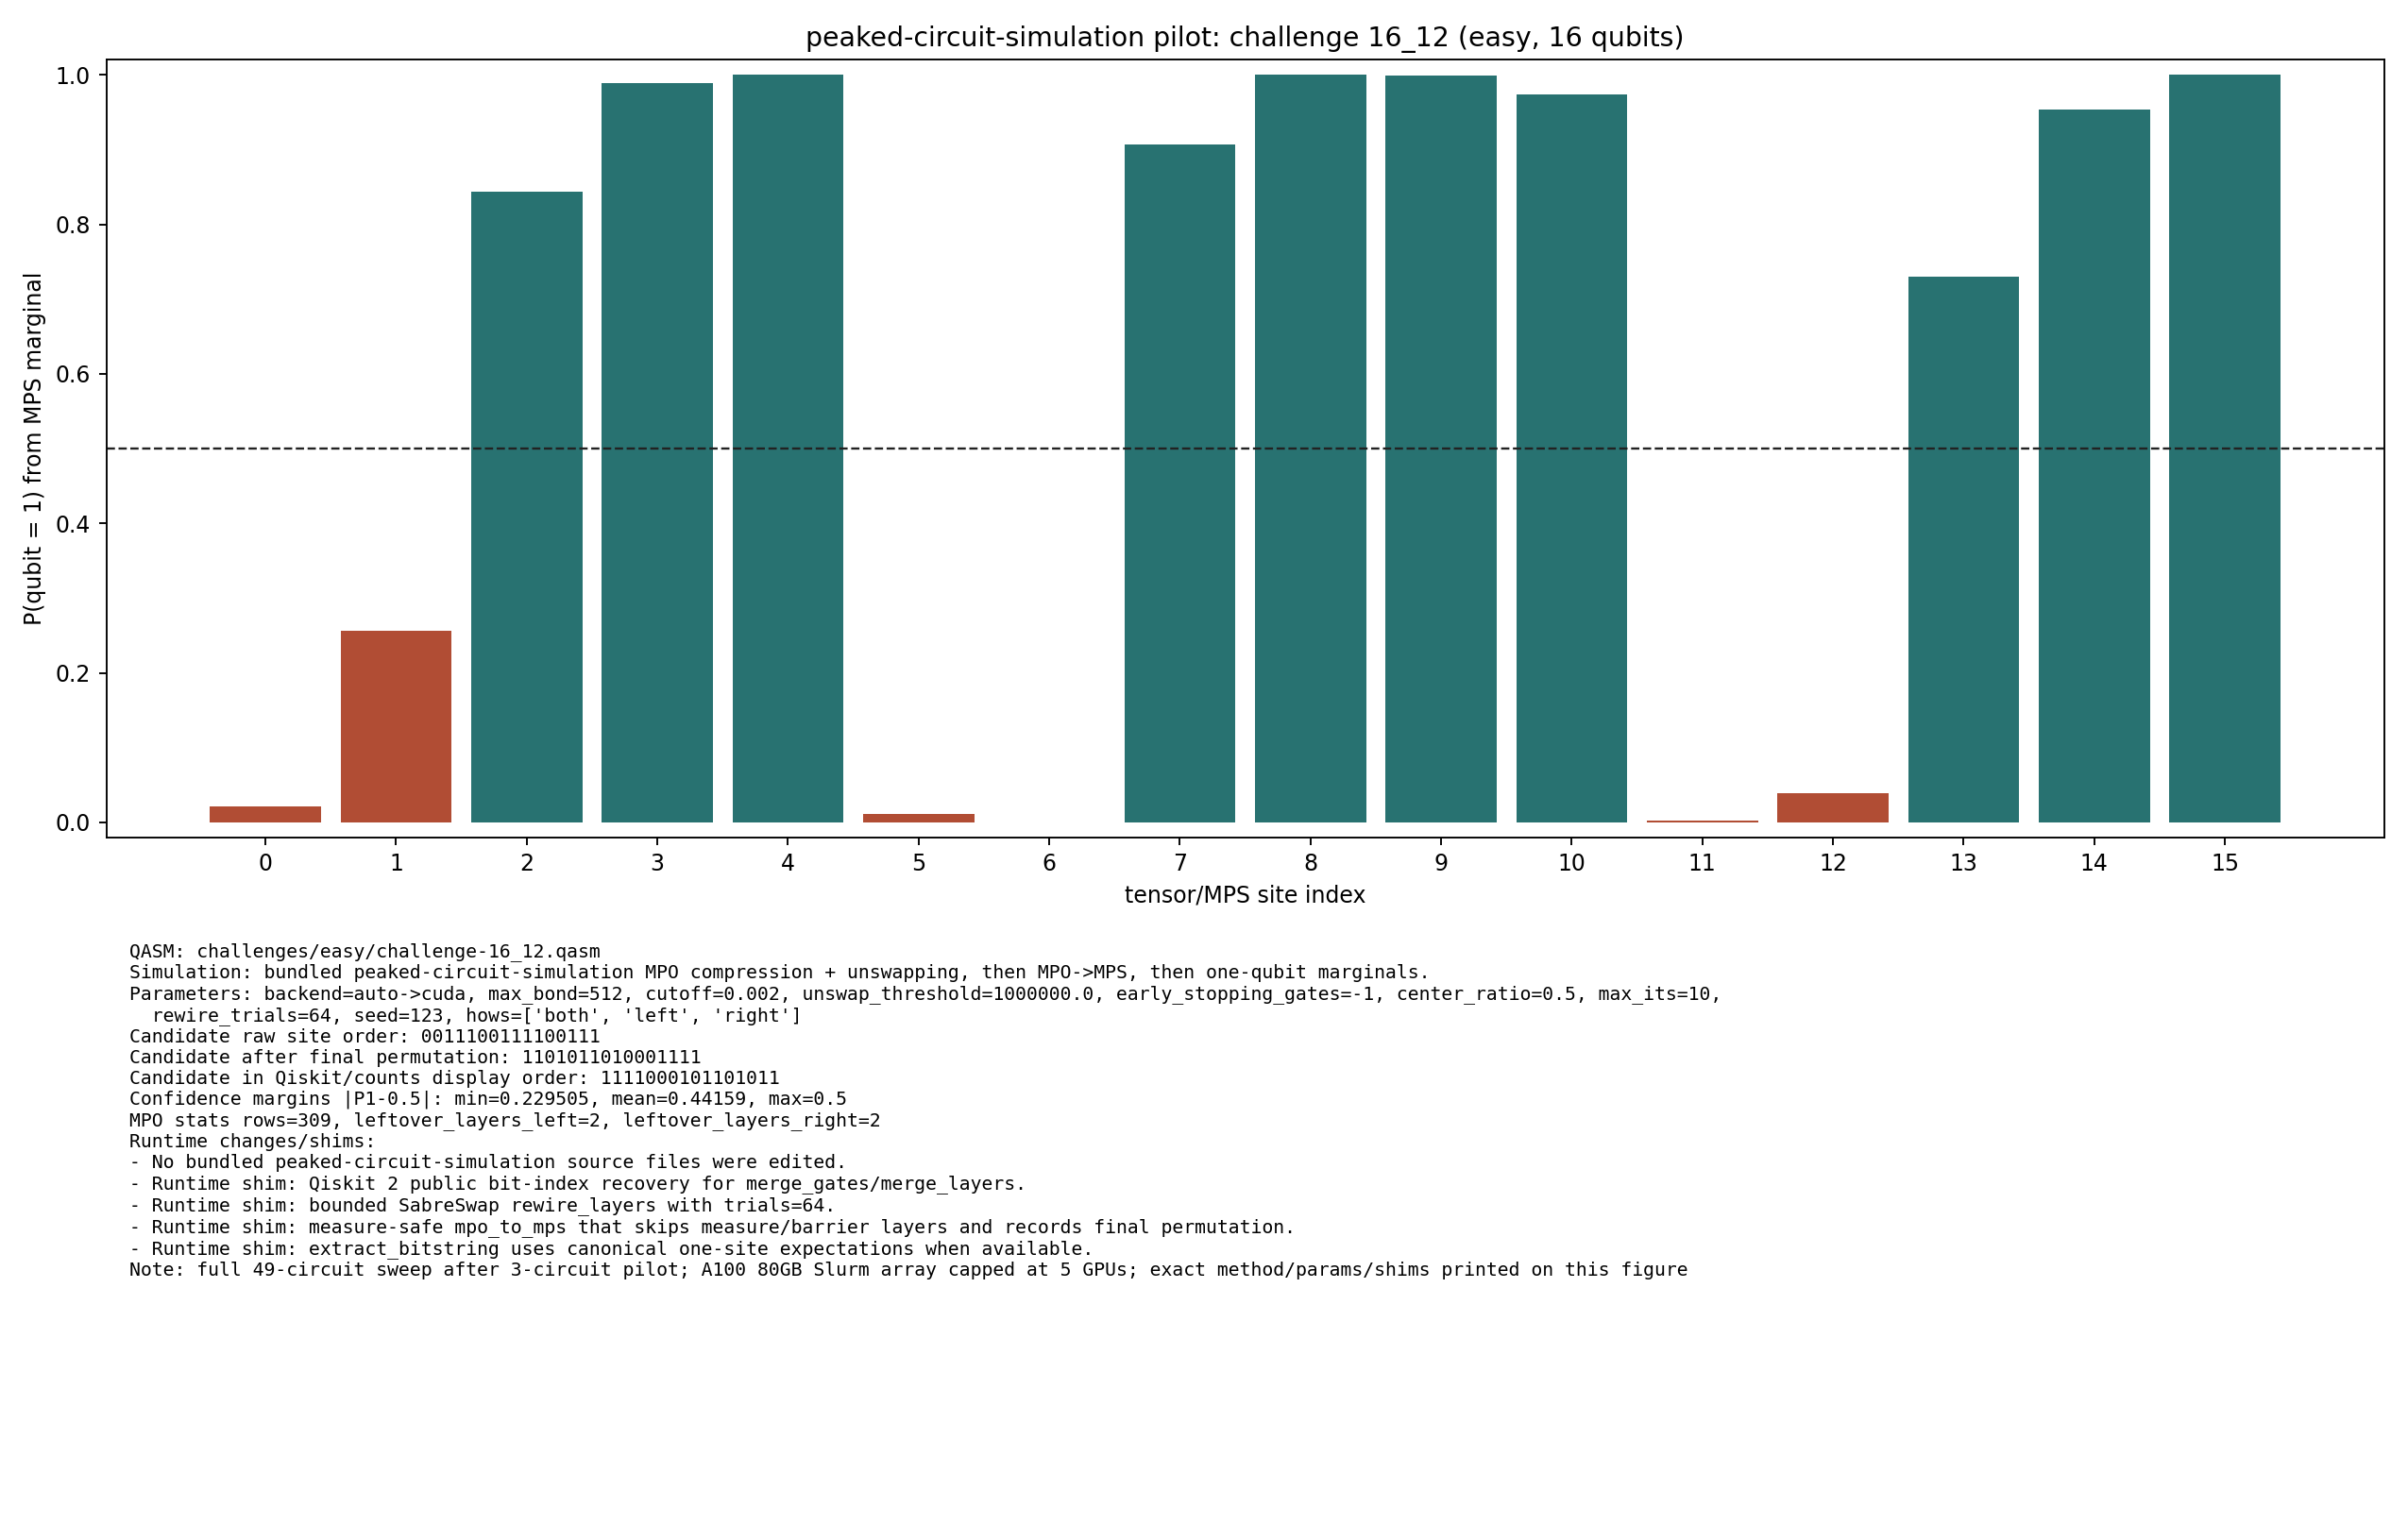
\includegraphics[width=\linewidth]{figures/peaked_16_12.png}
    \caption*{\code{16\_12}: matched exact, healthy margin.}
  \end{minipage}\hfill
  \begin{minipage}{0.32\linewidth}
    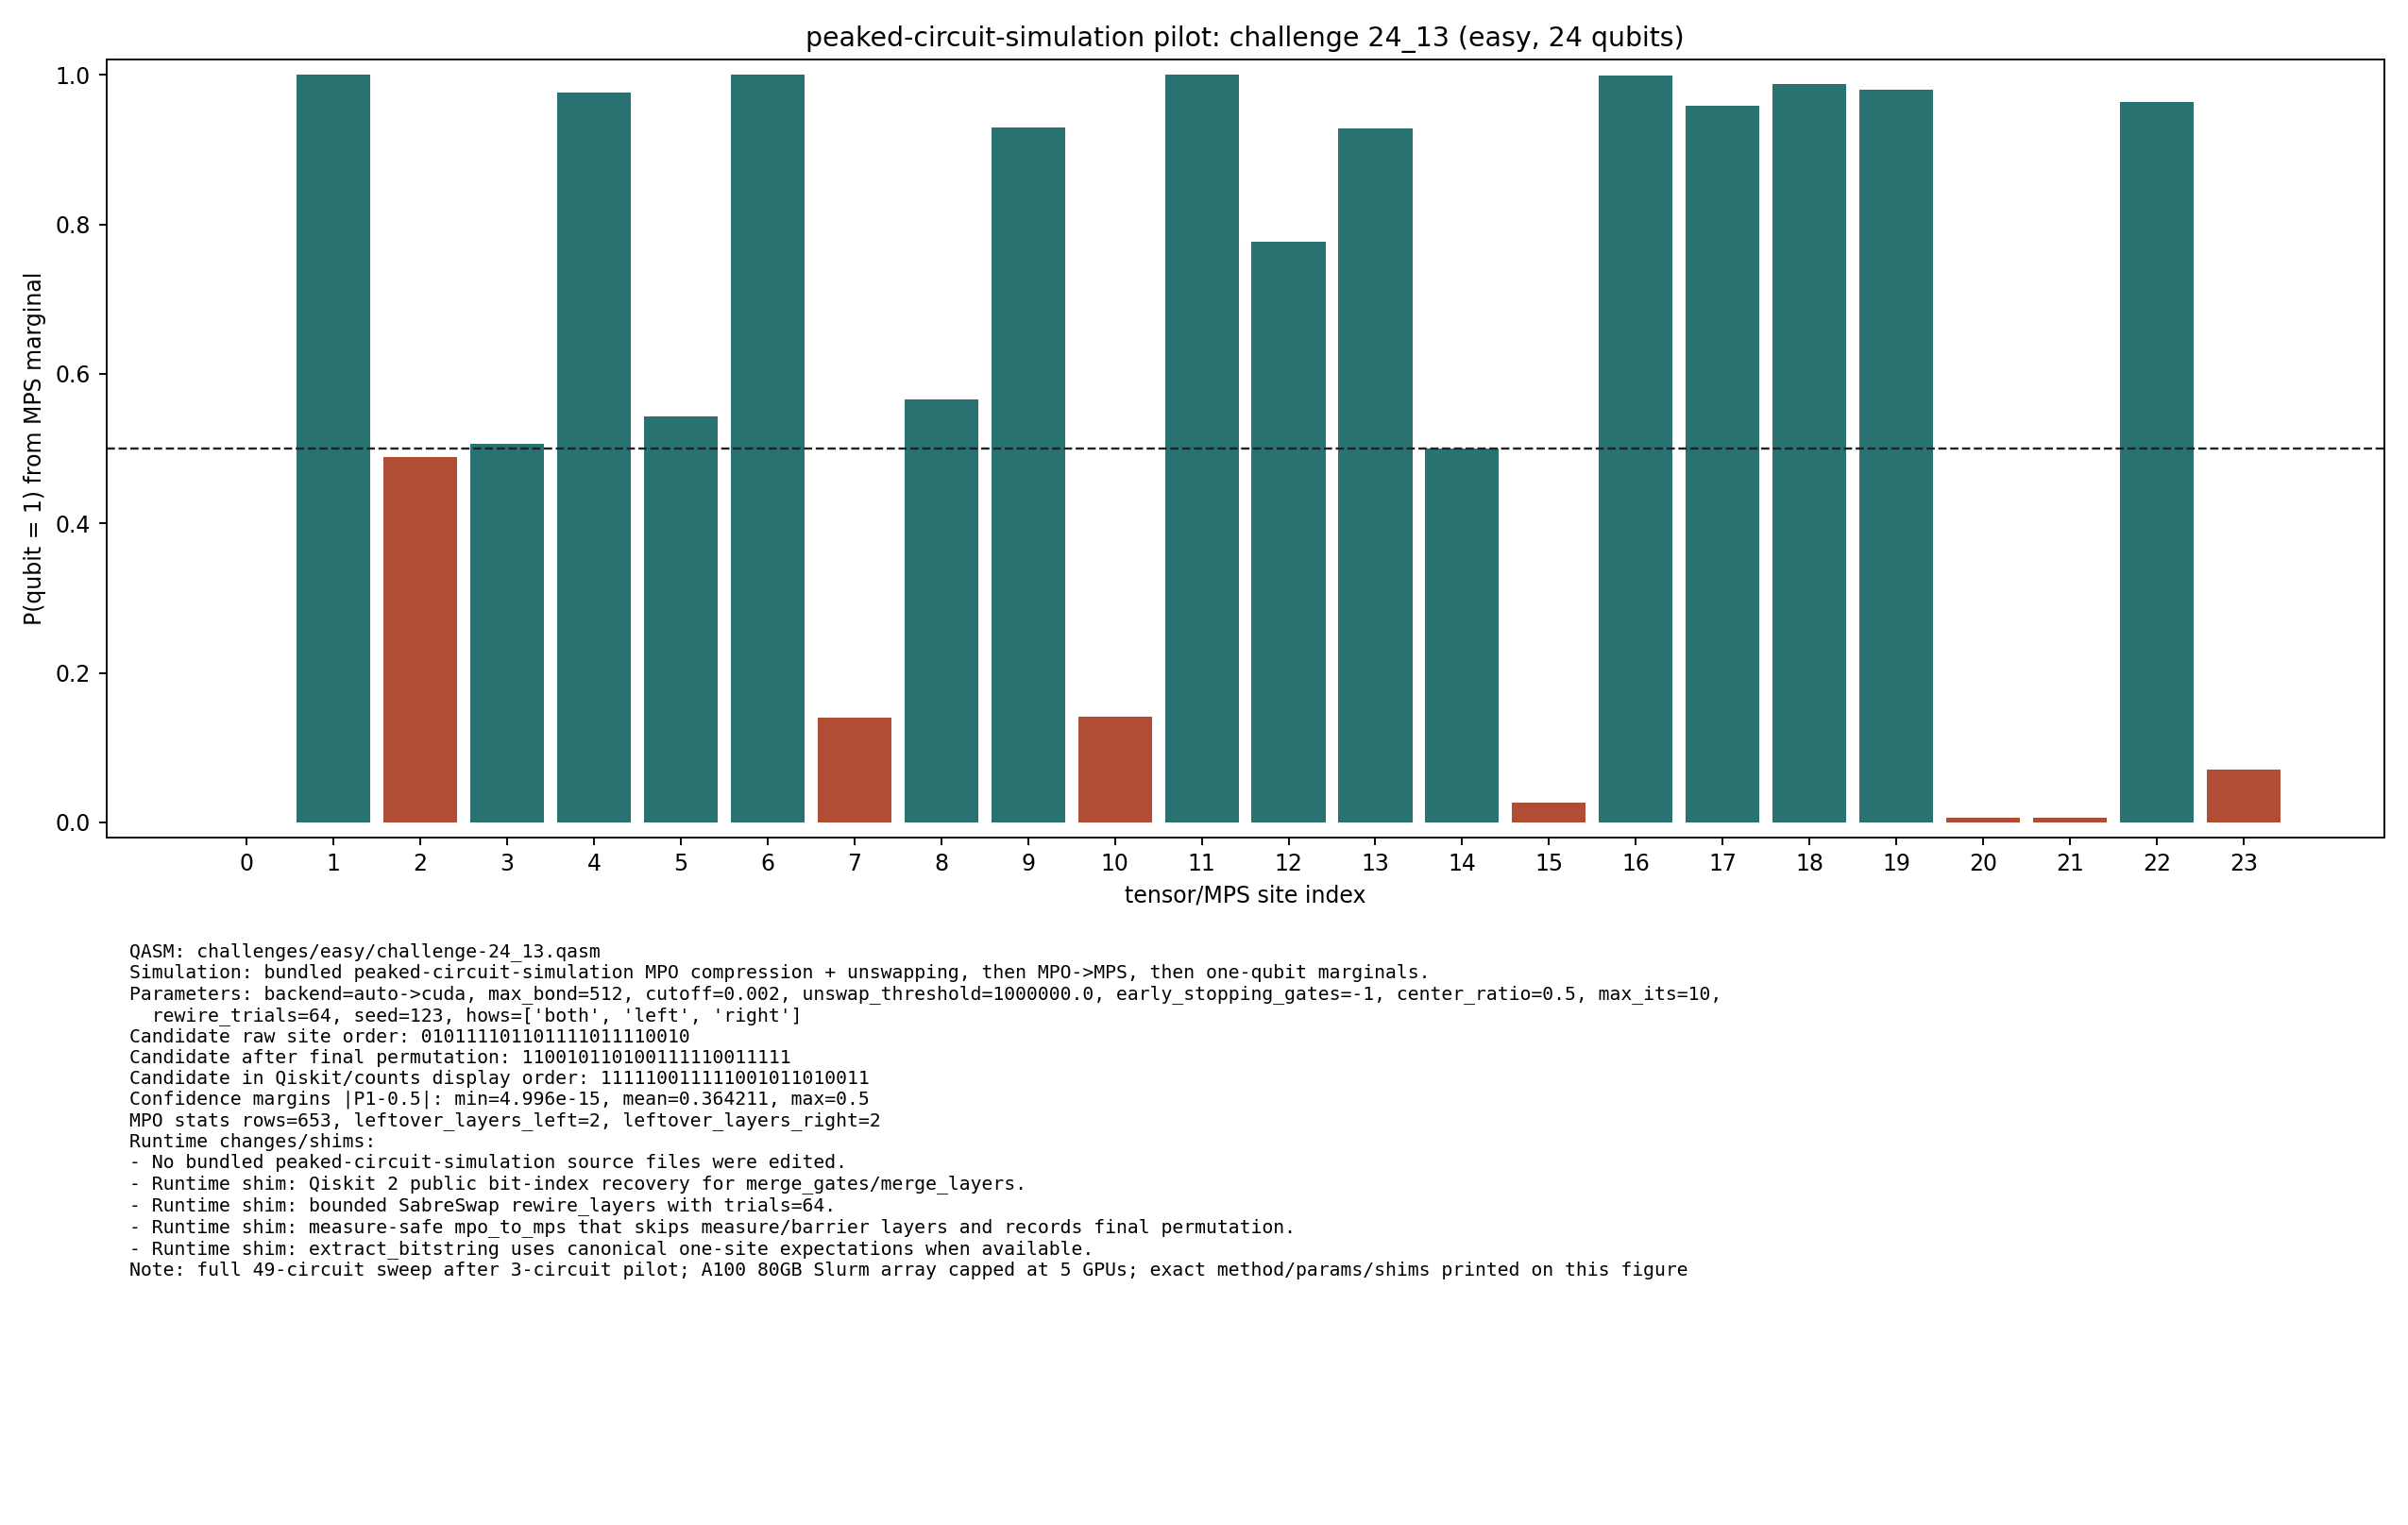
\includegraphics[width=\linewidth]{figures/peaked_24_13.png}
    \caption*{\code{24\_13}: one-bit miss.}
  \end{minipage}\hfill
  \begin{minipage}{0.32\linewidth}
    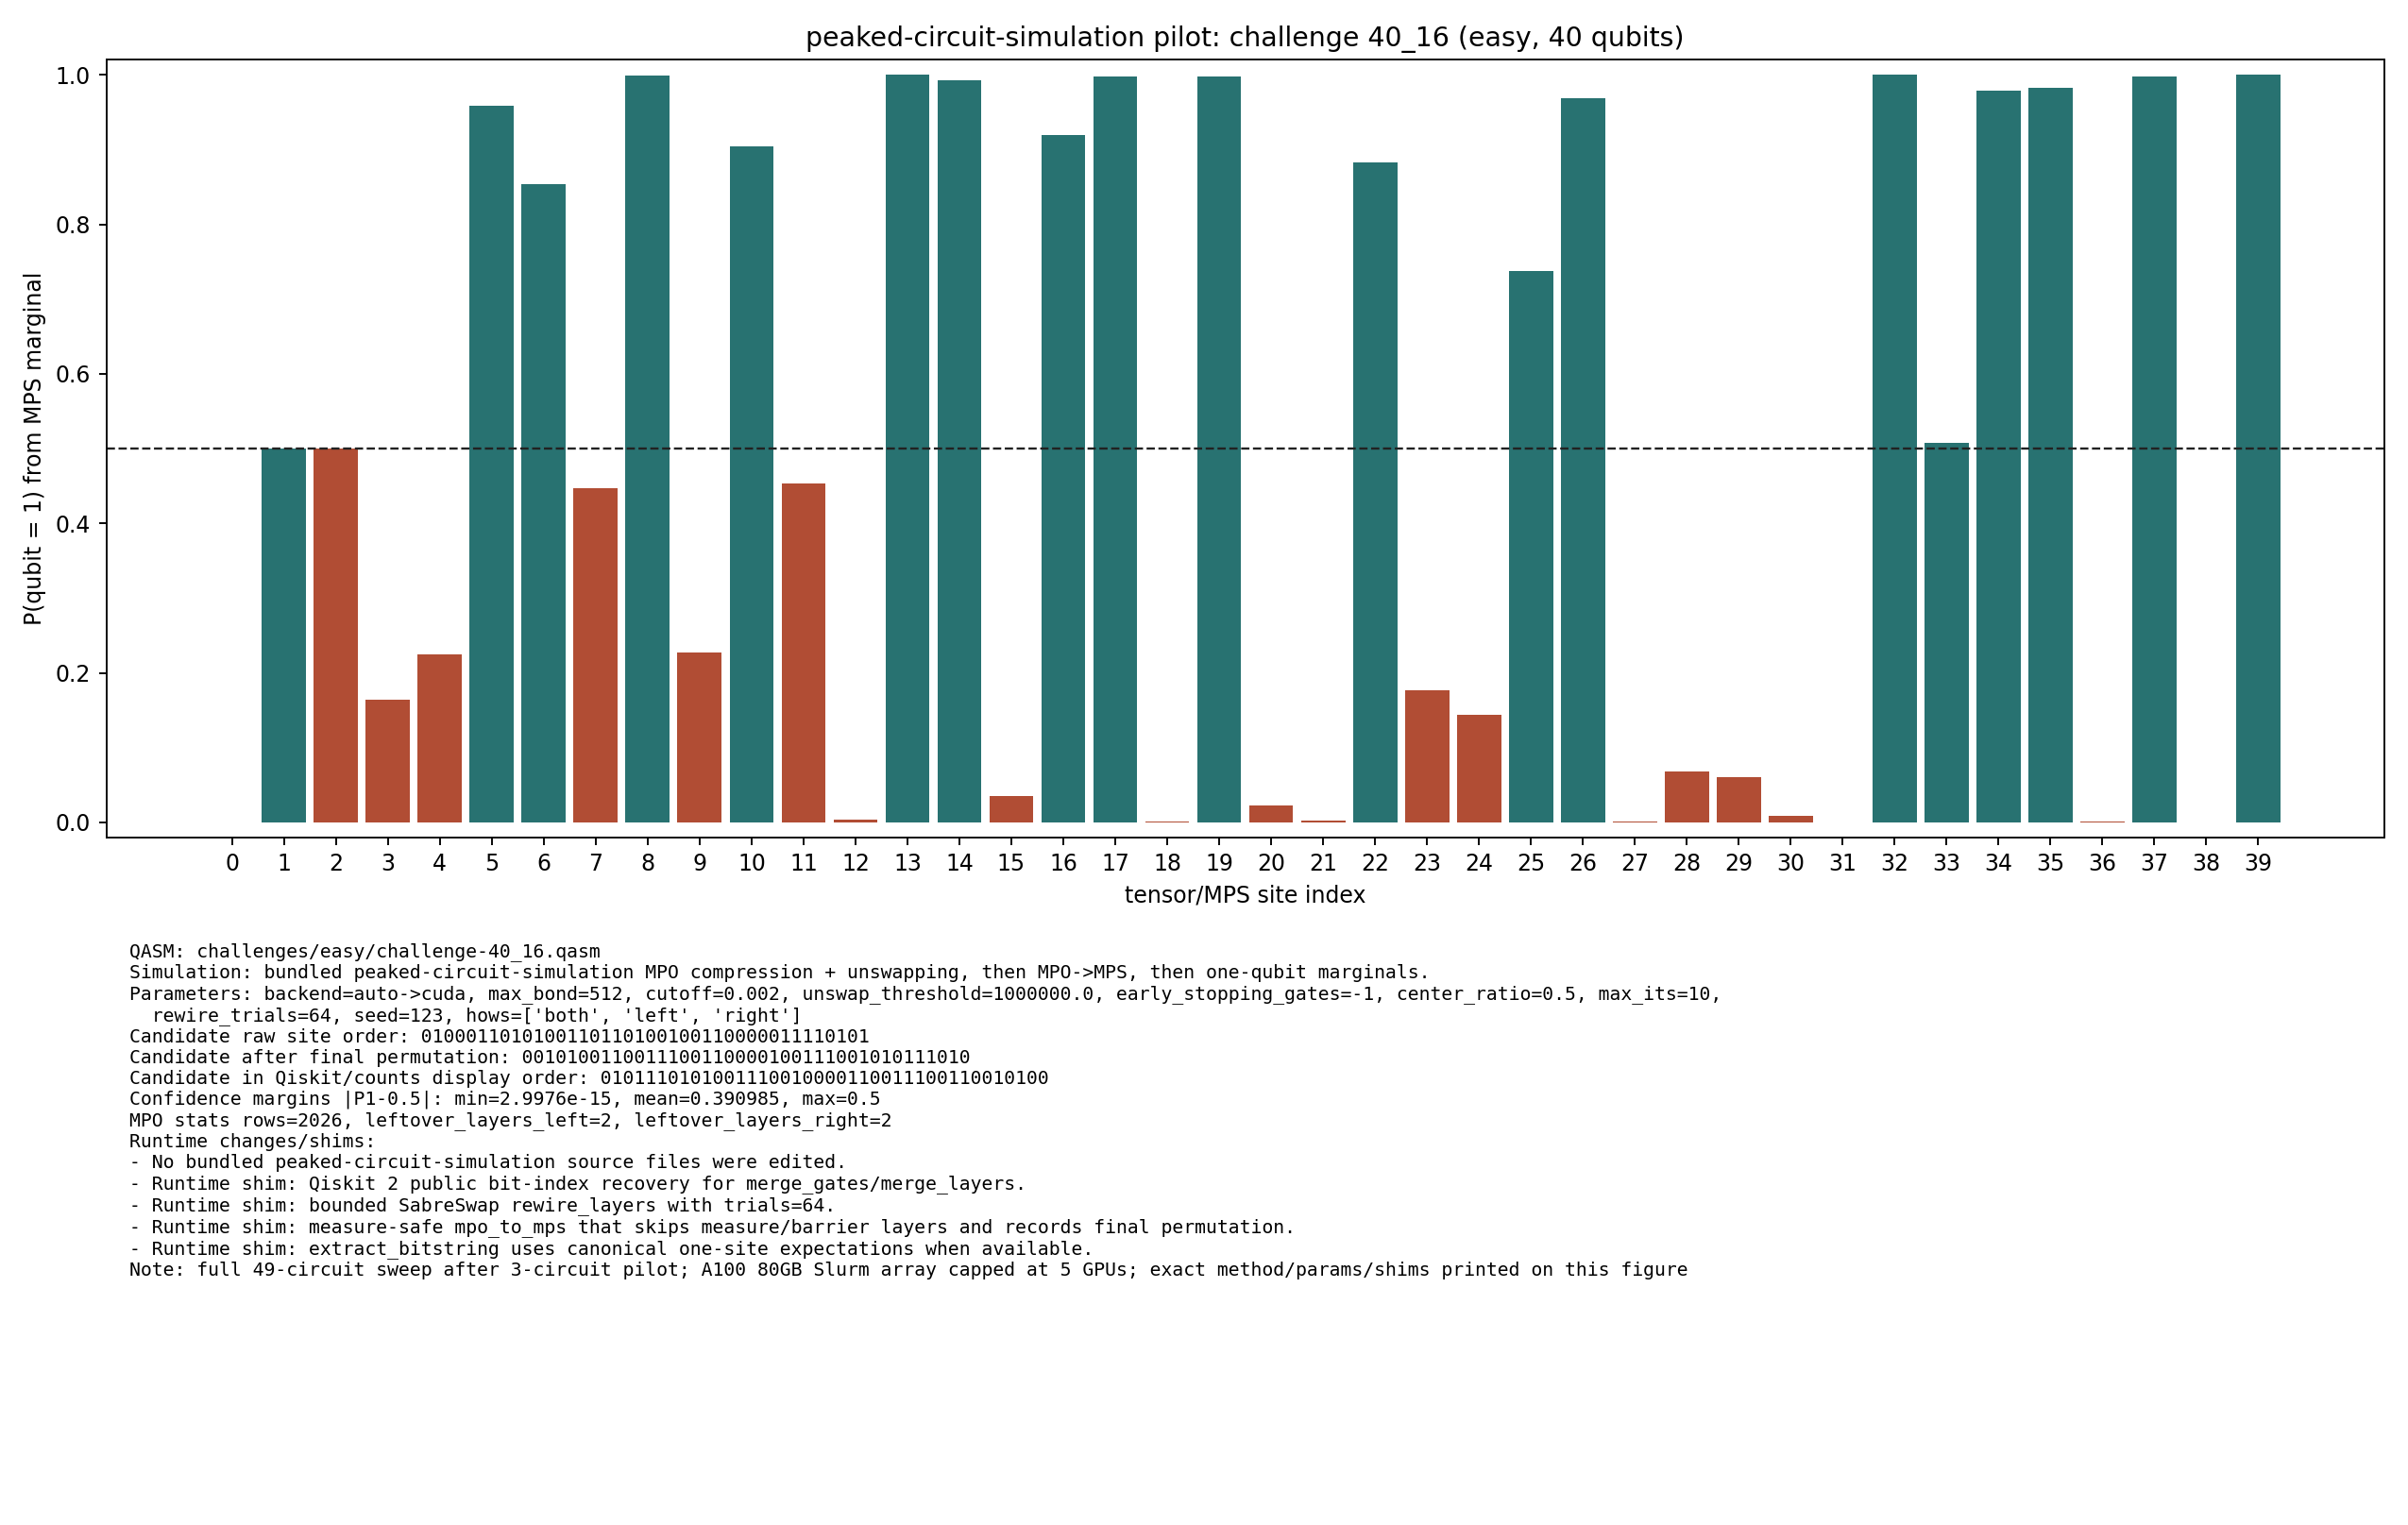
\includegraphics[width=\linewidth]{figures/peaked_40_16.png}
    \caption*{\code{40\_16}: disagrees with stable MPS distill.}
  \end{minipage}
  \caption{Representative peaked-circuit marginal plots.  The images were generated by the runner and include method/parameter annotations.}
\end{figure}

\begin{tabular}{llrp{0.43\linewidth}rr}
\toprule
Challenge & Difficulty & Qubits & Peaked candidate & Min margin & MPS bond \\
\midrule
16\_12 & easy & 16 & \bitstr{1111000101101011} & 2.30e-01 & 4 \\
24\_13 & easy & 24 & \bitstr{111110011111001011010011} & 5.00e-15 & 7 \\
32\_14 & easy & 32 & \bitstr{00000111001101000101110111101100} & 8.25e-05 & 4 \\
36\_15 & easy & 36 & \bitstr{101000011011111010101100111011001100} & 3.23e-03 & 6 \\
40\_16 & easy & 40 & \bitstr{0101110101001110010000110011100110010100} & 3.00e-15 & 4 \\
40\_17 & easy & 40 & \bitstr{0010010101010111001001000010001000001001} & 5.74e-05 & 4 \\
40\_18 & easy & 40 & \bitstr{1110010011010011000001010001010101100011} & 4.63e-13 & 6 \\
48\_19 & easy & 48 & \bitstr{011001010111101100111110000001011101001110010000} & 5.66e-15 & 3 \\
48\_20 & easy & 48 & \bitstr{010111000101001011110000100000011000010000010010} & 1.01e-07 & 3 \\
56\_22 & easy & 56 & \bitstr{11100100100110010011110010110110011000000100010111111011} & 4.53e-01 & 2 \\
56\_23 & easy & 56 & \bitstr{10100011000000101011101011011110111101110010000010000001} & 6.00e-13 & 4 \\
8\_11 & easy & 8 & \bitstr{01001110} & 2.10e-01 & 4 \\
\bottomrule
\end{tabular}


\subsection{Why \code{24\_13} Failed}
The \code{24\_13} exact statevector peak is
\begin{center}
\bitstr{111110011111001011010001}
\end{center}
with probability 0.591248.  The peaked MPO/MPS run emitted
\begin{center}
\bitstr{111110011111001011010011},
\end{center}
which differs in the second bit from the right, i.e. qubit $q_1$.

This was not a genuine ambiguity in the exact circuit.  Exact statevector gives $P(q_1=1)=0.0265$, so the bit should clearly be 0.  The compressed MPS/marginal extraction estimated the mapped marginal as $P(q_1=1)\approx0.5068$, barely above the threshold, and therefore flipped the bit.  The wrong candidate has exact probability about 0.01089 and rank roughly 12, so the failure was due to lossy compression/order-sensitive marginal extraction rather than a close second peak.

\section{Cross-Method Validation and Answer Selection}
The selection rule that emerged is:
\begin{enumerate}
  \item Use exact statevector answers whenever available.
  \item For non-exact circuits, prefer candidates repeated across seeds, shot counts, and bond dimensions.
  \item Down-rank any one-qubit marginal answer with minimum margin near zero.
  \item Treat all-unique MPS samples as samples only, not peak evidence.
  \item For serious submission candidates, the next validation should estimate probabilities of a short candidate set directly rather than relying on one full distribution.
\end{enumerate}

\begin{figure}[H]
  \centering
  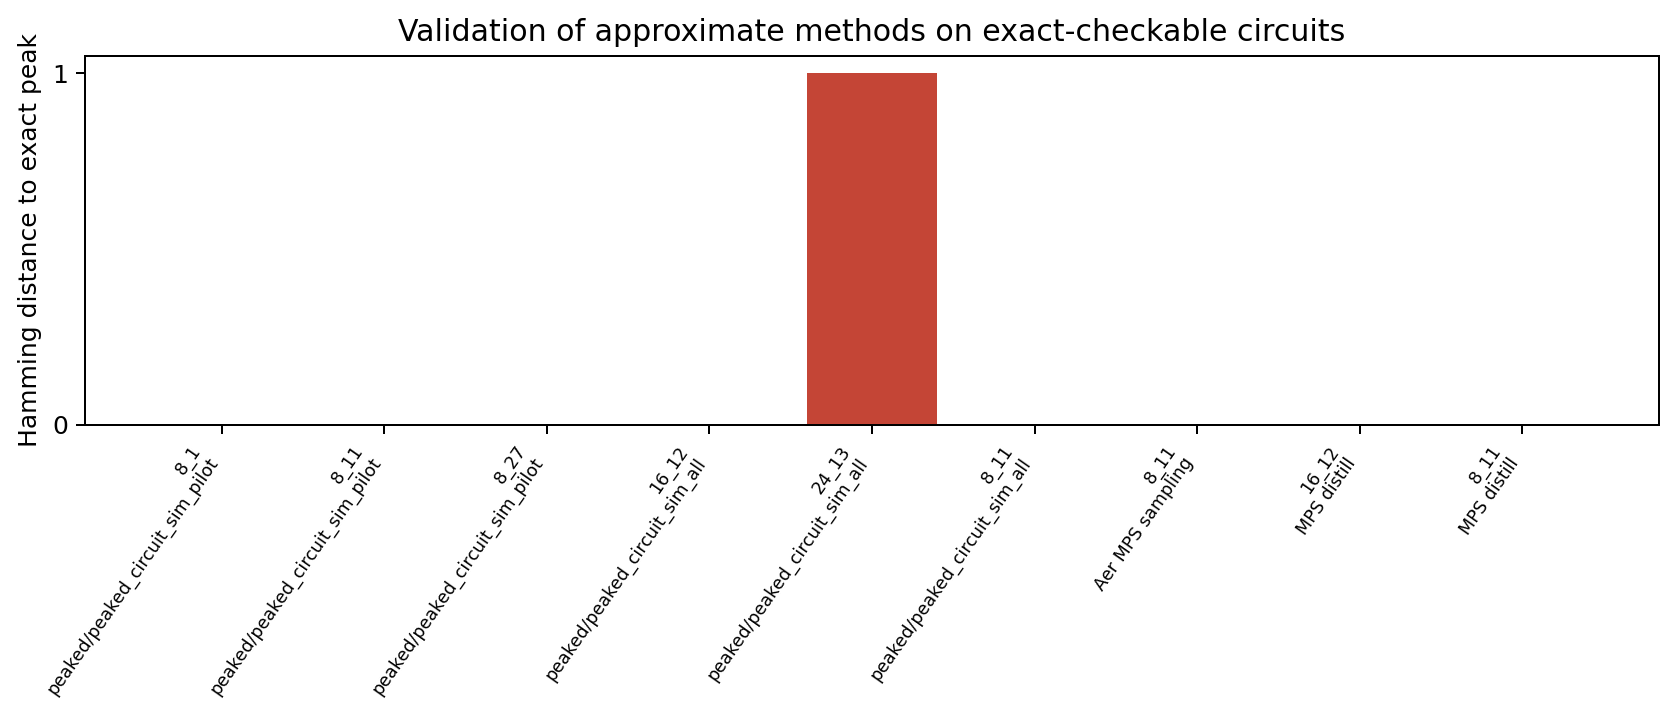
\includegraphics[width=0.9\linewidth]{figures/method_agreement.png}
  \caption{Approximate-method validation against exact baselines.  The only confirmed mismatch was \code{24\_13} from the peaked marginal method.}
\end{figure}

\begin{longtable}{p{0.10\linewidth}p{0.15\linewidth}p{0.39\linewidth}p{0.12\linewidth}p{0.18\linewidth}}
\caption{Candidate bitstrings and confidence after this session.}\\
\toprule
Challenge & Source & Candidate & Confidence & Reason \\
\midrule
\endfirsthead
\toprule
Challenge & Source & Candidate & Confidence & Reason \\
\midrule
\endhead
8\_1 & exact/peaked & \bitstr{10101101} & validated & Exact peak p=0.9126; peaked matched. \\
8\_11 & exact/peaked/MPS & \bitstr{01001110} & validated & All methods matched; exact p=0.5454. \\
8\_27 & exact/peaked & \bitstr{11001001} & validated & Exact p=0.2879; peaked matched. \\
16\_12 & exact/peaked/MPS & \bitstr{1111000101101011} & validated & All methods matched; exact p=0.4665. \\
24\_13 & exact & \bitstr{111110011111001011010001} & validated & Peaked marginal output was one bit off. \\
40\_16 & MPS distill & \bitstr{0101110101001110011000111011100110010110} & strong candidate & Stable across 6/6 MPS trials; peaked disagreed by 3 bits. \\
64\_26 & Aer MPS & \bitstr{0110101010100011010111011000011100010110110110011100011001100110} & candidate & Top count 287/4096; runner candidate only. \\
64\_34 & Aer MPS & \bitstr{0011010100010011001110101110100101001011001011011001111011100110} & candidate & Top count 552/4096; runner candidate only. \\
64\_41 & MPS samples & -- & unreliable & 4096/4096 unique in selected run; distill unstable. \\
104\_49 & MPS samples & -- & unreliable & 1024/1024 unique; no repeated peak evidence. \\
\bottomrule
\end{longtable}


\section{Current Conclusions}
The exact answers for small circuits are reliable.  The \code{peaked-circuit-simulation} method is promising but the current marginal-threshold version is not submission-safe without validation: it matched several exact circuits but missed \code{24\_13}, and it disagreed with a stable MPS-distilled \code{40\_16} candidate.  For larger problems, the best current candidates are \code{40\_16}, \code{64\_26}, and \code{64\_34}; \code{64\_41} and \code{104\_49} remain low confidence because sampled counts were flat.

Recommended next work:
\begin{itemize}
  \item Resubmit the incomplete peaked sweep only after the Slurm cancellation issue is understood.
  \item Add candidate probability evaluation: contract or sample around a small candidate set instead of extracting only one-qubit marginals.
  \item Continue higher-shot/higher-bond MPS distillation for hard circuits, requiring repeated winners across seeds.
  \item Pursue tree/tensor-network decompositions separately for nonlocal pairings and very-hard dense circuits.
\end{itemize}

\begin{thebibliography}{9}
\bibitem{gharibyan2025}
H. Gharibyan et al.,
\emph{Heuristic Quantum Advantage with Peaked Circuits}, arXiv:2510.25838, 2025.

\bibitem{kremerdupuis2025}
D. Kremer and E. Dupuis,
\emph{Efficient Classical Simulation of Heuristic Peaked Quantum Circuits}, arXiv:2604.21908, 2025.

\bibitem{rudolphtindall2025}
M. Rudolph and J. Tindall,
\emph{Simulating and Sampling from Quantum Circuits with 2D Tensor Networks}, arXiv:2507.11424, 2025.
\end{thebibliography}

\end{document}
